\documentclass[../main.tex]{subfiles}

\begin{document}
	
	\subsection{Generación y validación de resúmenes modelo}
	
	Con el objetivo de evaluar la calidad de los resúmenes generados automáticamente, se elaboró un conjunto de resúmenes modelo que sirvieron como referencia en el proceso de validación.
	
	Estos resúmenes se generaron a partir de historiales médicos anonimizados combinados con una instrucción común, que especificaba el estilo y el nivel de detalle esperado. Tanto los historiales como la instrucción fueron preparados previamente en archivos de texto plano para facilitar su procesamiento.
	
	Para la generación automática de los resúmenes se empleó la API de OpenAI, utilizando el modelo gpt-4o-mini en modo de procesamiento por lotes (batch). Este modo permite enviar múltiples solicitudes en un solo envío, lo que resulta especialmente útil cuando se trabaja con grandes volúmenes de datos. Cada solicitud incluía un historial clínico y el prompt correspondiente \parencite{openaiBatch}.
	
	Una vez enviado el lote, se monitorizó su estado hasta que todas las respuestas estuvieron disponibles, las cuales fueron posteriormente organizadas y vinculadas con sus respectivos historiales originales.
	
	Finalmente, una muestra de los resúmenes generados fue revisada por profesionales del Hospital Clínico Universitario de Málaga, con el objetivo de que confirmasen que los textos resultantes contenían la información relevante de forma clara y adecuada, validando así su uso como referencia en la evaluación del sistema.
	
	
	\subsection{Comparación de modelos SLM con resúmenes de referencia}
	
	Tras generar un conjunto de resúmenes modelo utilizando la API de OpenAI, se evaluó el rendimiento de distintos modelos de lenguaje de menor tamaño con el objetivo de determinar qué modelos eran capaces de aproximarse con mayor fidelidad a los resúmenes de referencia generados por GPT-4o-mini. Además, se midió el tiempo de inferencia de cada modelo.
	
	\subsubsection{Modelos utilizados}
	
	Los modelos de la tabla \ref{tab:modelos} se ejecutaron localmente mediante la herramienta ollama, que permite la interacción con modelos preentrenados de forma eficiente y a alto nivel. Ya que el objetivo de este trabajo es utilizar la cantidad mínima de cómputo, la ventaja más notable de esta herramienta es que implementa automáticamente el particionado del modelo entre GPU y CPU (conocido en inglés como offloading) si es necesario.
	
	\begin{table}[h]
		\centering
		\caption{Lista de modelos utilizados en el proyecto.}
		\label{tab:modelos}
		\renewcommand{\arraystretch}{1.2}
		\begin{tabular}{cccc}
			\hline
			\textbf{Modelo} & \textbf{Parámetros}& \textbf{Tamaño de ventana} & \textbf{Cuantización} \\
			\hline
			qwen:14b & 14b & 32768 tokens & Q4\_0 \\
			llama3.1 & 8b & 131072 tokens & Q4\_K\_M  \\
			llama3.2 & 3b & 131072 tokens & Q4\_K\_M  \\
			deepseek-r1:14b & 14b & 131072 tokens & Q4\_K\_M \\
			deepseek-r1:8b & 8b & 131072 tokens & Q4\_K\_M \\
			mistral & 7b & 32768 tokens & Q4\_0 \\
			phi4 & 14b & 16384 tokens & Q4\_K\_M  \\
			\hline
		\end{tabular}
	\end{table}
	
	
	Para cada historial clínico, se utilizaron diferentes contextos o instrucciones del sistema, almacenadas en archivos de texto, que se incorporaron como mensajes del sistema al inicializar el modelo. Se evaluaron dos configuraciones distintas de temperatura (0.2 y 0.8) para estudiar su efecto en la generación de texto. 
	
	
	\subsubsection{Técnicas de Prompting utilizadas}
	
	Durante las pruebas realizadas con distintos modelos de lenguaje, se aplicaron diversas metodologías de prompting con el objetivo de optimizar la calidad de las respuesta. A continuación se detallan las principales estrategias empleadas, junto con su justificación:
	
	\begin{itemize}
		\item \textbf{Template-based prompting}: Se diseñaró una plantilla con la estructura que debe tener el resumen. Esta técnica, al ser consistente en contenido fue usada en la obtención de resúmenes modelos en el paso anterior. Esta técnica permite estandarizar el formato de entrada y aprovechar estructuras de lenguaje que los modelos ya han visto durante su entrenamiento \parencite{brown2020languagemodelsfewshotlearners}. 
		
		\item \textbf{Chain-of-Thought (CoT)}: Se utilizó esta estrategia para inducir razonamiento complejo. De esta forma se mejora la capacidad para resolver problemas en etapas, especialmente en tareas lógico-matemáticas o de toma de decisiones secuencial \parencite{wei2023chainofthoughtpromptingelicitsreasoning}.
		
		\item \textbf{Few-shot prompting}: Se introdujo un ejemplo dentro del prompt para mejorar la generalización del modelo en tareas específicas. Los modelos de lenguaje suelen tener buenos resultados si tienen ejemplos a seguir \parencite{parnami2022learningexamplessummaryapproaches}.
		
		\item \textbf{Stepwise refinement}: Esta técnica consistió en dividir tareas complejas en subtareas más pequeñas que eran resueltas en etapas consecutivas. Se aplicó principalmente cuando el modelo cometía errores por falta de planificación en tareas extensas. Su efectividad ha sido destacada en investigaciones sobre razonamiento iterativo \parencite{sun2024promptchainingstepwiseprompt}.
		
		\item \textbf{Generación por partes}: Dado que algunos modelos tienen ventanas de contexto limitadas (por ejemplo, 4k tokens), se optó por dividir la entrada y salida en bloques lógicos. Hacer resúmenes de partes del historial y juntarlos en uno resulta costoso pero puede hacer que se mantenga coherencia en textos largos \parencite{press2023measuringnarrowingcompositionalitygap}.
	\end{itemize}
	
	
	\subsubsection{Evaluación automática}
	
	Las respuestas generadas fueron comparadas con las respuestas de referencia mediante dos tipos de métricas automáticas comúnmente utilizadas en tareas de procesamiento de lenguaje natural:
	
	\begin{itemize}
		\item \textbf{BLEU} (Bilingual Evaluation Understudy): mide la superposición de n-gramas entre la respuesta generada y la esperada. Se utilizó la variante con suavizado de Chencherry \parencite{papineni-etal-2002-bleu}.
		\item \textbf{ROUGE} (Recall-Oriented Understudy for Gisting Evaluation): se calcularon las variantes ROUGE-1, ROUGE-2 y ROUGE-L, que capturan la coincidencia de unigramas, bigramas y la subsecuencia más larga común respectivamente \parencite{lin-2004-rouge}.
		\item \textbf{BERTScore}: mide la similitud semántica entre la respuesta generada y la referencia utilizando los embeddings contextuales de BERT. Calcula la similitud coseno entre los vectores de las palabras en ambos textos, y se reportan las métricas de precisión, recuerdo y F1 \parencite{zhang2020bertscoreevaluatingtextgeneration}.
		
	\end{itemize}
	
	Estas fueron implementadas usando las bibliotecas nltk y rouge-score de Python.
	


\subsection{Implementación del modelo final}
\subsubsection{RAG}

Una vez seleccionado el mejor modelo, se buscó optimizar aún más su rendimiento mediante la implementación de un sistema de Retrieval-Augmented Generation (RAG).

Este enfoque consistió en proporcionar contexto adicional al modelo a partir de una base de datos de preguntas y respuestas médicas, con el objetivo de mejorar la precisión en la tarea de resumir historias clínicas. Aunque este método se emplea comúnmente en aplicaciones de asistencia conversacional, ha demostrado ser eficaz también en la generación de resúmenes clínicos \parencite{ALKHALAF2024104662}.

Se utilizó un conjunto de datos compuesto por 194,000 preguntas y respuestas del dataset MEDMCQA \parencite{pmlr-v174-pal22a}, las cuales fueron transformadas en vectores de embeddings y almacenadas en una base de datos vectorial utilizando ChromaDB.

La Figura \ref{fig:diagrama_rag} presenta el diagrama de flujo del sistema implementado, que sigue los siguientes pasos:

\begin{enumerate}
	\item El historial clínico se divide en secciones, siguiendo el mismo esquema empleado en la generación por partes, para facilitar una búsqueda ordenada de información.
	\item Se solicita al modelo que identifique las ideas principales de cada sección del texto, con el fin de usarlas como claves de búsqueda.
	\item Cada una de estas ideas se consulta en la base de datos vectorial, obteniendo definiciones o respuestas a preguntas relacionadas.
	\item A continuación, se resume cada sección del historial clínico, incorporando como contexto la información obtenida en el paso anterior.
	\item Finalmente, los resúmenes parciales se fusionan utilizando el modelo para generar un resumen consolidado de la historia clínica.
\end{enumerate}

\begin{figure}[H]
	\centering
	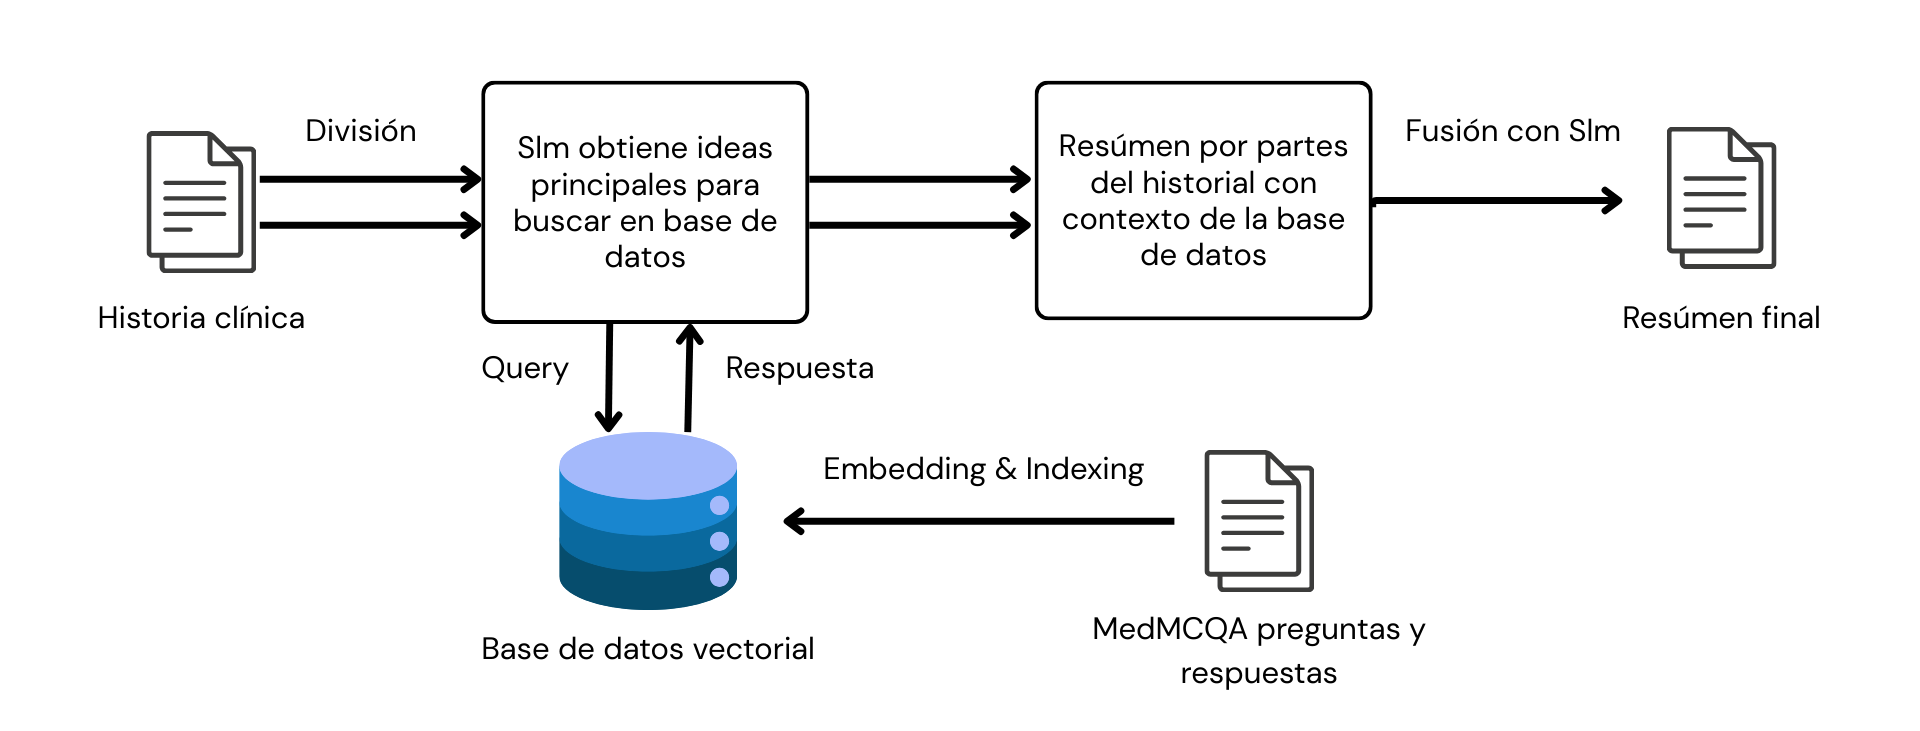
\includegraphics[width=0.8\textwidth]{images/diagrama-flujo-rag.png}
	\caption{Diagrama de flujo del sistema RAG.}
	\label{fig:diagrama_rag}
\end{figure}
\subsubsection{Ajuste fino del modelo}

Debido a las limitaciones en los recursos computacionales disponibles, se optó por ajustar el modelo más pequeño entre los evaluados, específicamente el llama3.2:3b-instruct, aplicando una cuantización de 4 bits para reducir el uso de memoria y facilitar el entrenamiento en hardware limitado.

La cuantización es una técnica que reduce la precisión de los parámetros del modelo, disminuyendo así su tamaño y los requisitos de memoria. En particular, la cuantización a 4 bits permite representar los pesos del modelo utilizando solo 4 bits por valor, en lugar de los 32 bits típicos en punto flotante. Esto resulta en una compresión significativa del modelo, permitiendo su ejecución en dispositivos con recursos limitados \parencite{huggingface_4bit}.

Para ajustar el modelo cuantizado, se empleó la técnica de Low-Rank Adaptation (LoRA), que introduce adaptadores de bajo rango en las capas del modelo. Esta metodología permite modificar solo una pequeña fracción de los parámetros, manteniendo el resto del modelo congelado, lo que reduce considerablemente los requisitos computacionales y de memoria durante el entrenamiento \parencite{hu2021lora}.

El proceso de ajuste fino se llevó a cabo utilizando la biblioteca Unsloth, una herramienta de código abierto diseñada para facilitar y optimizar el entrenamiento de modelos de lenguaje grandes en entornos con recursos limitados. Unsloth proporciona implementaciones eficientes de técnicas como LoRA y cuantización, y maneja automáticamente la gestión de memoria y el procesamiento de datos durante el entrenamiento \parencite{unsloth_docs}.

Uno de los desafíos más significativos fue comprender y aplicar correctamente las plantillas de prompts. Estas plantillas definen la estructura de las entradas que se proporcionan al modelo durante el entrenamiento y la inferencia, y son cruciales para guiar el comportamiento del modelo de manera coherente. La correcta implementación de estas plantillas asegura que el modelo interprete y responda adecuadamente a las instrucciones proporcionadas \parencite{huggingface_templates}.

El entrenamiento se realizó utilizando Unsloth con los siguientes parámetros:

\begin{itemize}
	\item Número de ejemplos: 256,916
	\item Épocas: 1
	\item Tamaño de batch por dispositivo: 2
	\item Pasos de acumulación de gradiente: 4
	\item Tamaño total de batch: 8
	\item Parámetros entrenables: 24,313,856 de un total de 3,000,000,000 (0.81\% del modelo)
	\item Tiempo total de entrenamiento: aproximadamente 6 minutos
\end{itemize}

Durante el entrenamiento, Unsloth gestionó de manera eficiente la memoria, descargando gradientes según fuera necesario para optimizar el uso de VRAM.

Los datos utilizados para el ajuste fino provienen del repositorio ruslanmv/ai-medical-chatbot \parencite{ruslanmv2024aimedchatbot}, que contiene un conjunto de datos especializado en conversaciones médicas. Este conjunto de datos proporcionó ejemplos relevantes para adaptar el modelo a tareas específicas en el ámbito de la medicina.



\subsection{Desarrollo de la aplicación web demostrativa}

Como parte de la validación práctica del sistema propuesto, se ha desarrollado una aplicación web simple que permite interactuar con el modelo de lenguaje entrenado. Esta aplicación permite introducir un historial clínico y obtener como respuesta un resumen generado automáticamente.

\subsubsection{Tecnologías utilizadas}

\begin{itemize}
    \item \textbf{FastAPI}: framework de backend utilizado para definir la API REST que comunica al usuario con el modelo.
    \item \textbf{Ollama}: herramienta para ejecutar modelos de lenguaje localmente de forma eficiente.
    \item \textbf{HTML, CSS y JavaScript}: usados para construir la interfaz web de forma sencilla y funcional.
\end{itemize}

\subsubsection{Endpoints de la API}

La API cuenta con los siguientes endpoints:

\begin{itemize}
    \item POST /predict: recibe un historial médico en formato texto plano y devuelve el resumen generado por el modelo.
    \item GET /: endpoint que sirve los archivos estáticos (HTML, CSS y JavaScript) de la web.
\end{itemize}

\subsubsection{Funcionamiento general}

Cuando el usuario envía un historial médico desde el formulario web, este se envía al endpoint /predict. El backend lo procesa y consulta al modelo cargado en Ollama, que genera la respuesta. Esta es devuelta al usuario en la misma página web.



\end{document}